



%Autor: Nico Schrodt
%Oktober 2021 - Mai 2022


\documentclass[12pt]{article}

\usepackage{multicol}
\usepackage{geometry}
\usepackage{blindtext}
\usepackage{setspace}
\usepackage{hyperref}
\usepackage[headsepline=0.8pt, footsepline =0.8pt]{scrlayer-scrpage}
\usepackage{listings}
\usepackage{subcaption}
\usepackage{tabularx}
\usepackage{xurl} %Formats \url{}-entrys better
\usepackage{color, colortbl}
%\usepackage{pdfpages}
\usepackage{amssymb}

\geometry{a4paper, top=25mm, left=35mm, right=25mm, bottom=25mm, headsep=13mm, footskip=12mm, head=14.5pt}

%encoding
%--------------------------------------
\usepackage[utf8]{inputenc}
\usepackage[T1]{fontenc}
%--------------------------------------

%German-specific commands
%--------------------------------------
\usepackage[ngerman]{babel}
%--------------------------------------

%Hyphenation rules
%--------------------------------------
\usepackage{hyphenat}
%--------------------------------------

\usepackage{graphicx}
\graphicspath{ bilder/}

\newcommand{\Autor}{Nico Schrodt}

\newcommand{\Bearbeitungszeitraum}{5 + 6 Semester}
\newcommand{\Kurs}{TINF19B3}
\newcommand{\Betreuer}{Daniel Lindner}

\newcommand{\DHBWLogoDeckblatt}{
\includegraphics[width=4.5cm]{Logos/dhbw-logo}}

\newcommand{\Titel}{Entwerfen und Implementieren einer Verschlüsselungssoftware}
\newcommand{\ArtArbeit}{Ausarbeitung}
\newcommand{\Abschluss}{Bachelor of Science}
\newcommand{\Studiengang}{Studiengang Informationstechnik}

\newcommand{\Ort}{Karlsruhe}

%\newcommand{\Abgabedatum}{16.02.2021}


\begin{document}
\onehalfspacing
\pagenumbering{Roman}
	\begin{titlepage}
		{\DHBWLogoDeckblatt}\\[2cm]
		\begin{center}
			\vspace*{-2cm}
			{\Huge \Titel}\\[2cm]
			{\Huge \ArtArbeit}\\[2cm]
			{\Large \Abschluss}\\[0.5cm]
			{\large \Studiengang}\\[0.5cm]
			{\large an der}\\[0.5cm]
			{\large Dualen Hochschule Baden-Württemberg Karlsruhe}\\[0.5cm]
			{\large von}\\[0.5cm]
			{\large\bfseries \Autor}\\[1cm]
			{\large Abgabedatum \today}
			\vfill
		\end{center}
		\begin{tabular}{l@{\hspace{1cm}}l}
			Bearbeitungszeitraum & \Bearbeitungszeitraum \\
			Kurs & \Kurs \\
%			Ausbildungsfirma & \Ausbildungsfirma \\
			Dozent & \Betreuer \\
		\end{tabular}
	\end{titlepage}

\newpage

\thispagestyle{empty}
\tableofcontents

\newpage

%\thispagestyle{empty}
%\thispagestyle{plain}
%\cleardoublepage
%\addcontentsline{toc}{section}{\listfigurename}
%\listoffigures

%\addcontentsline{toc}{section}{\listtablename}
%\listoftables

%\addcontentsline{toc}{section}{Listings}
%\lstlistoflistings

%\newpage

%\thispagestyle{empty}
%\thispagestyle{plain}
%\cleardoublepage
%\section*{Abkürzungsverzeichnis}
%\addcontentsline{toc}{section}{Abkürzungsverzeichnis}

%\newpage
\pagenumbering{arabic}

%% Kopf und Fusszeilen==================================================== 
\pagestyle{scrheadings} % Seite mit Headern 

% loescht voreingestellte Stile 
\clearpairofpagestyles
%\clearscrheadings 
\clearmainofpairofpagestyles
%\clearscrplain 

% %%% Kopfzeile 
% einseitig: Bei einseitigem Layout, nur folgende Zeilen verwenden !!! 
%\ohead[] {
\includegraphics[height=0.5cm]{Logos/Firmenlogokopfzeile}}
\ihead[]{\leftmark} % links: Kapitel
%\chead[]{} % mitte: 

% %%% Fusszeile 
%\cfoot[]{} % mitte: 
\cfoot[\pagemark]{\pagemark} % rechts: Seitenzahl


% Angezeigte Abschnitte im Header 
\automark{section}  % Inhalt von [\rightmark]{\leftmark} 

\section{Einführung}
Dieses Kapitel befasst sich vorwiegend mit relevanten Grundlagen der Arbeit. Unter anderem wird das Ziel spezifiziert, elementare Aspekte der Arbeitsweise eines Prozessors werden erläutert und die verschiedenen Werkzeuge mit denen das Ziel realisiert wird werden aufgeführt.

\subsection{Ziel der Arbeit}
In dieser Arbeit soll ein Simulationsprogramm geschrieben werden, mit dem mehrere unterschiedliche 8-Bit Prozessoren simuliert werden können. Dazu sollen die Grundlegenden Eigenschaften in kurzen Lernprogrammen erläutert werden. Ebenfalls soll es eine interaktive Einweisung geben wie der Simulator verwendet werden kann.

\subsection{Repository}
Der Quellcode kann in folgendem GitHub-Repository abgerufen werden:\\ \url{https://github.com/NicoSchrodt/EncryptionService}

\subsection{Commit-Historie}
Der Titel jedes Kapitels hat eine Fußnote die den Commit angibt während dem das Kapitel geschrieben wurde bzw. dieses zuletzt verändert wurde. Für Abschnitte in denen auf spezifische Änderungen eingegangen wird, werden i.d.R eigene Commits angegeben mit direktem Link (100\% RickRoll-Frei, für paranoide ist der Commit auch seperat angegeben).

\noindent{\Huge Sollte dieser Satz noch hier sein: Dies ist eine Vorabversion als Notfalls falls ich vergessen habe die fertige Version rechtzeitig hochzuladen.\par}

\subsection{UML-Diagramm}
\begin{center}
	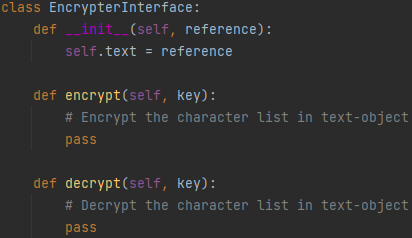
\includegraphics[width=10cm]{bilder/Decorator_before.png}
\end{center}
\newpage

\section{Clean Architecture}
Der Sinn einer Clean Architecture ist es das Programm in klar definierte Schichten zu zerlegen die unabhängig voneinander ausgetauscht werden können. Dadurch soll idealerweise die Langlebigkeit und Wartbarkeit eines Projekts gewährleistet werden können.

\subsection{Geplante Schichtenarchitektur}
Für dieses Projekt sind zwei Schichten vorgesehen. Einmal die Benutzeroberfläche (GUI) welche mit Qt implementiert wird und die Logik, welche unter anderem die Verschlüsselung vornimmt. Der Benutzer soll ausschließlich mit der von Qt generierten Oberfläche interagieren z.B. durch Textfelder oder Knöpfe, welche vorkonfigurierte Befehle ausführen.

\subsection{Umsetzung}
Platzhalter

\subsubsection{Benutzeroberfläche}
Platzhalter

\subsubsection{Verschlüsselungsdienst}
Platzhalter

\newpage

\section{Entwurfsmuster}
Das für den Umfang dieses Programmentwurfs verwendete Entwurfsmuster ist der Dekorierer. Aufgabe des Dekorierers ist es eine Klasse oder Funktion um einen oder mehrere Aspekte zu erweitern ohne die Klasse selbst zu verändern. Das Entwurfsmuster wurde in der Klasse 'EncrypterInterface.py' angewendet.
\begin{center}
	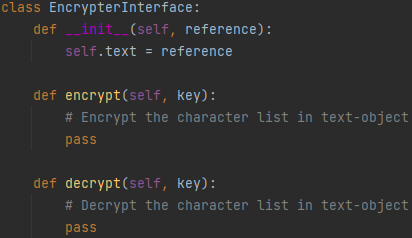
\includegraphics[width=10cm]{bilder/Decorator_before.png}
\end{center}
'EncrypterInterface' dient wie der Name bereits verrät als Interface für konkrete Encrypter. Dabei ist aber nicht gewährleistet, dass die konkrete Implementierung die im Interface beschriebenen Funktion selbst implementiert. Der Dekorierer soll hier die Aufgabe Übernehmen, auf eine konkrete Implementierung zu kontrollieren und bei Fehlen dieser eine Exception auszulösen.
\begin{center}
	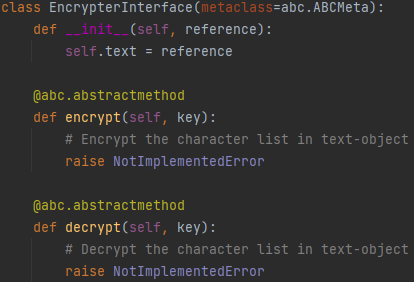
\includegraphics[width=10cm]{bilder/Decorator_after.png}
\end{center}
Die Funktion des Dekorierers beschränkt sich hier auf konkrete Implementierungen des EncrypterInterfaces, Also Klassen die von 'EncrypterInterface' erben. Das Interface selbst könnte potentiell immer noch instantiiert und verwendet werden ohne die Exception auszulösen.

\newpage

\section{Programming Principles}
In diesem Abschnitt werden kurz einige Programming Principles erläutert und deren Anwendung an Beispielen in diesem Projekt aufgezeigt.

\subsection{SOLID}
\subsubsection{Single Responsibility Principle}
Das Single Responsibility Principle steht für die Anforderung das jede Klasse nur eine einzige Aufgabe bzw. Verantwortung haben soll. Sinn dahinter ist es Komplexität und unerwünschte Kopplung zu vermeiden. Generell ist nämlich davon auszugehen das eine Klasse mit mehreren Verantwortungen Interaktionen zwischen diesen hat, was unter anderem das Ändern einzelner erschwert.
Als Beispiel dafür wird in der unteren Abbildung eine konkrete Implementierung der Encrypter Klasse hergezogen.
\begin{center}
	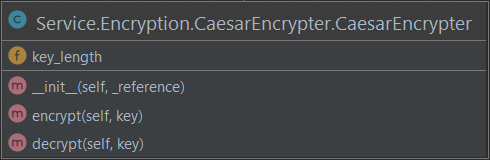
\includegraphics[width=10cm]{bilder/SRP.png}
\end{center}
Die Klasse hat effektiv eine Aufgabe. Sie erhält bei Instanziierung ein Textobjekt. Auf diesem Textobjekt werden Verschlüsselungen durchgeführt, dabei wird lediglich zwischen Ver- und Entschlüsseln unterscheiden.

\subsubsection{Open/Closed Principle}
Das Open/Closed Principle beschreibt das Designziel Klassen, Funktionen, etc. so aufzubauen das sie offen sind für Erweiterungen und geschlossen für Veränderungen. Konkret heißt das, neue Anforderungen sollen eher durch z.B. Vererbung realisiert werden, statt konkreten Modifikationen in der relevanten Klasse. Dieses Prinzip wurde für das Projekt beispielsweise durch Vererbung realisiert. Statt einer generellen Encrypter-Klasse wird ein Interface verwendet, welches für jede verschiedene Anwendung eine davon erbende Klasse hat.
\begin{center}
	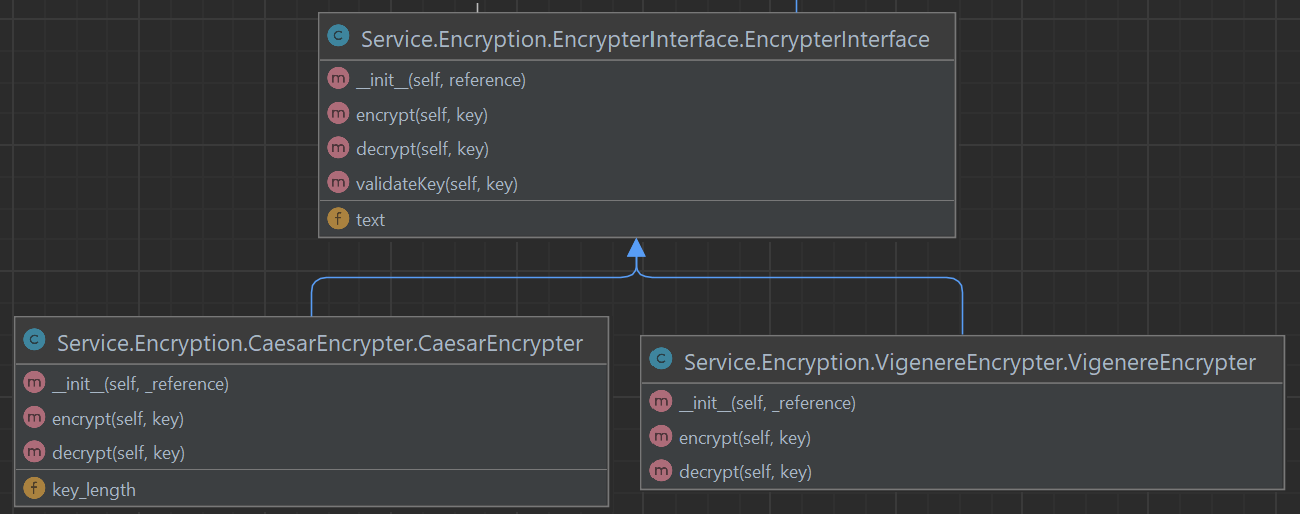
\includegraphics[width=10cm]{bilder/OCP.png}
\end{center}
Dadurch ist es möglich weitere Verschlüsselungen hinzuzufügen ohne das Interface oder die erbenden Klassen zu modifizieren.
\subsubsection{Liskov Substitution Principle}
Das Liskov Substitution Principle vermittelt das Prinzip, das jede Spezialisierung, z.B. durch Polymorphie bei Vererbung, an jeder Stelle verwendet werden können muss an der auch die Generalisierung verwendet wird. Beispielsweise soll also die Funktion einer Erbenden Klasse nicht zu einem Fehler führen an einer Stelle an der die Funktion der Ursprungsklasse funktioniert hat.
\begin{center}
	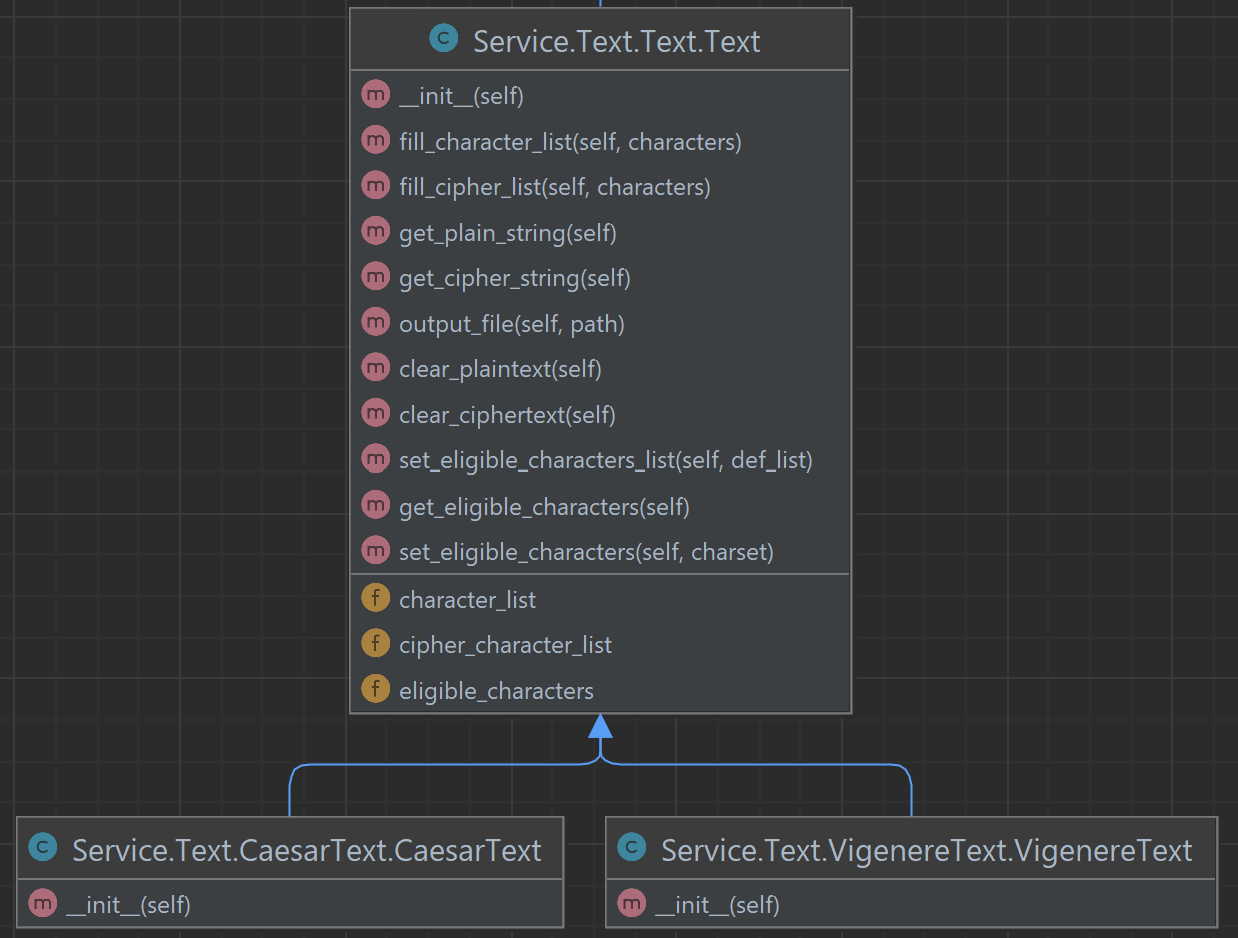
\includegraphics[width=10cm]{bilder/LSP.png}
\end{center}
Die Struktur an der dieses Prinzip Anwendung findet wäre in diesem Projekt die Text-Klasse sowie den Kindern dieser. Generell haben diese die selben Funktionen und können auch anstelle der Textklasse verwendet werden. Die Unterschiede liegen lediglich in der Instanziierung der Unterklassen, welche bspw. das Charset verändern.

\subsubsection{Interface Segregation Principle}
Mit dem Interface Segregation Principle soll verhindert werden, dass Klassen ein über-spezifiziertes Interface verwenden. Ein verwendetes Interface soll also möglichst schlank sein und nicht zu viele Funktionen auf einmal anbieten. Damit soll verhindert werden, dass Klassen Zugriff auf Funktionen haben die sie gar nicht verwenden.

\subsubsection{Dependency Inversion Principle}
Das Dependency Inversion Principle beschreibt effektiv das Prinzip der Entkopplung. Klassen auf einer höheren Ebene bspw. der Logik eines Programms solle nicht von niedrigeren Klassen z.B. Benutzerinterfaces abhängen. Dies wird unter anderem durch Verschieben der Abhängigkeit erreicht, bspw. auf ein Interface und dem Übergeben von Referenzen auf konkrete Instanzen.

\subsection{GRASP}

\subsubsection{Low Coupling}
'Low Coupling' oder 'Niedrige Kopplung' meint das Prinzip, dass Programmcode besser ist je weniger Abhängigkeiten auf die Umgebung bestehen bzw. diese möglichst nah beieinander sind. Das soll eine flexiblere Anwendung ermöglichen und Modifikationen erleichtern, da die Anzahl an Abhängigkeiten überschaubarer ist.

\subsubsection{High Cohesion}
'High Cohesion' oder ein hohes Maß an Kohäsion stellt das Gegenstück zur niedrigen Kopplung dar. Hierbei soll sichergestellt werden, dass 'naher' Code tatsächlich eng miteinander Arbeitet. Das kann sich z.B. darin widerspiegeln ob Code ein Klasse regelmäßig verwendet wird oder nur in Spezialfällen. Prinzipiell ist ein Weg dieses Ziel zu erreichen das Aufspalten von großen Klassen in Subklassen mit kleineren und spezifischeren Aufgaben. Im Projekt wird dies erreicht durch implementieren einzelner Klassen für jede Verschlüsselung statt einer großen 'Encrypter'-Klasse.
\begin{center}
	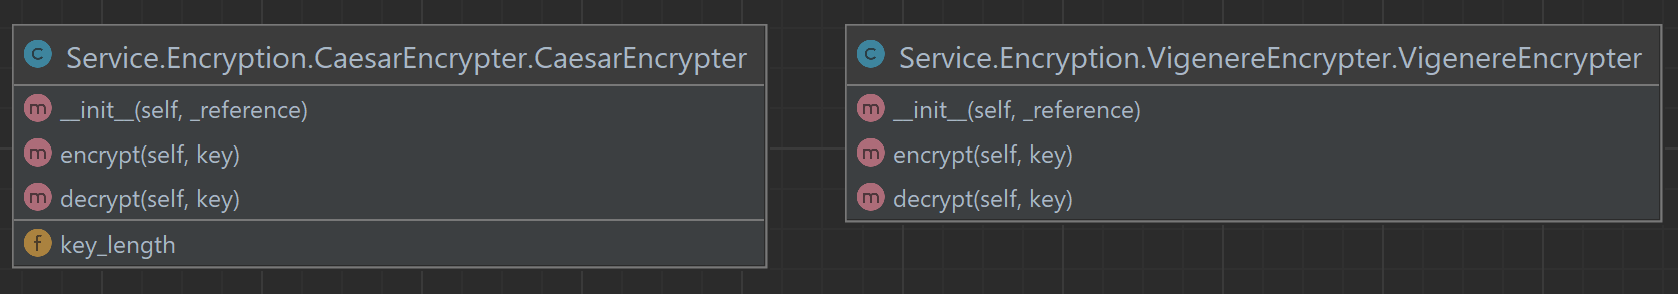
\includegraphics[width=10cm]{bilder/High_Cohesion.png}
\end{center}

\subsection{DRY}
DRY steht für 'Don't repeat yourself'. Zentraler Angelpunkt dieses Prinzips ist das Vermeiden von Code Duplikaten, sowie das Strukturieren des Programmcodes in einer Weise das nur logisch verknüpfte Elemente sich gegenseitig beeinflussen. Oder in anderen Worten, jedes logische Konstrukt im Quellcode muss durch eine klare von anderen Aspekten getrennte Struktur repräsentiert werden. Dadurch lassen sich z.B. einige Code Smells verhindern wie "Duplicated Code" oder "Shotgun Surgery".\\
Das Prinzip wurde angewendet hinsichtlich dem vermeiden von Code Duplikaten, welche sich unter anderem in zahlreichen Klassen die für die Verschlüsselung zuständig sind befanden, da der Prozess der Ver- und Entschlüsselung je nach Verfahren recht ähnlich ist (bspw. Vigenère- oder Caesar-Chiffre).

\newpage

\section{Refactoring}
Das Ziel von Refactoring ist das Verbessern der Codequalität. Für diese Arbeit ist es unterteilt in das Identifizieren von 3 verschiedenen Code Smells und das Anwenden von 2 Refactorings.

\subsection{Code Smells}
Unter 'Code Smells' versteht man Stellen im Programmcode, welche Verbesserungspotential aufweisen bspw. bezüglich der Übersichtlichkeit.\\ (\textbf{Anmerkung: }Die hier aufgelisteten Code Smells sind womöglich nicht mehr in der neuesten Version des Projekts zu finden, sondern nur noch in älteren Commits)

\subsubsection{Code Smells 1 Duplicated Code}
Dieses Beispiel für einen 'Duplicated Code'- Code Smells ist in der 'Caesar-Encrypter.py'- Datei zu finden. Ausschlaggebend ist hierbei, dass das Verfahren zum Ver- und Entschlüsseln effektiv gleich ist mit der Ausnahme, welcher der Starttext ist und in welche Richtung (Positiv/Negativ) der Schlüssel anzuwenden ist.
\begin{center}
	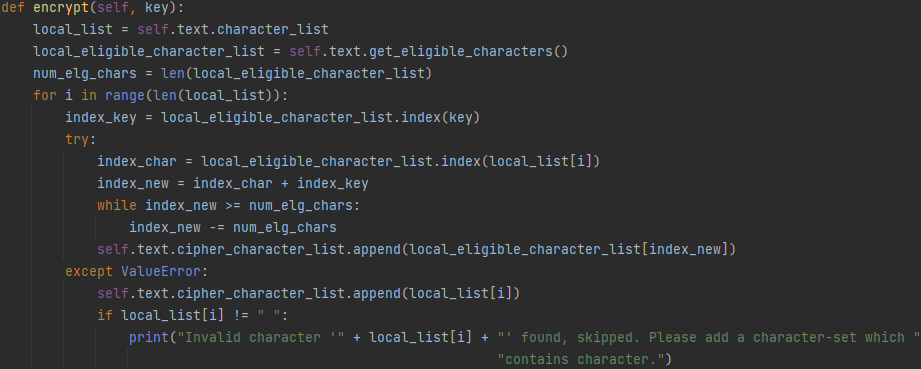
\includegraphics[width=15cm]{bilder/CodeSmells1_a.png}
\end{center}
\begin{center}
	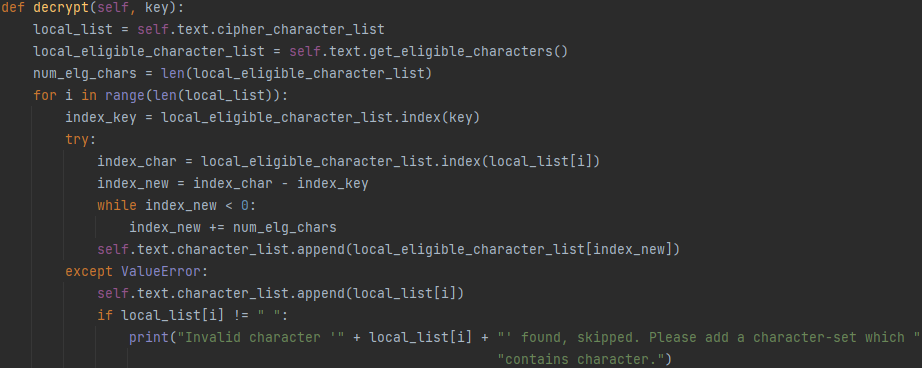
\includegraphics[width=15cm]{bilder/CodeSmells1_b.png}
\end{center}

\subsubsection{Code Smells 2 Long Method}
\begin{center}
	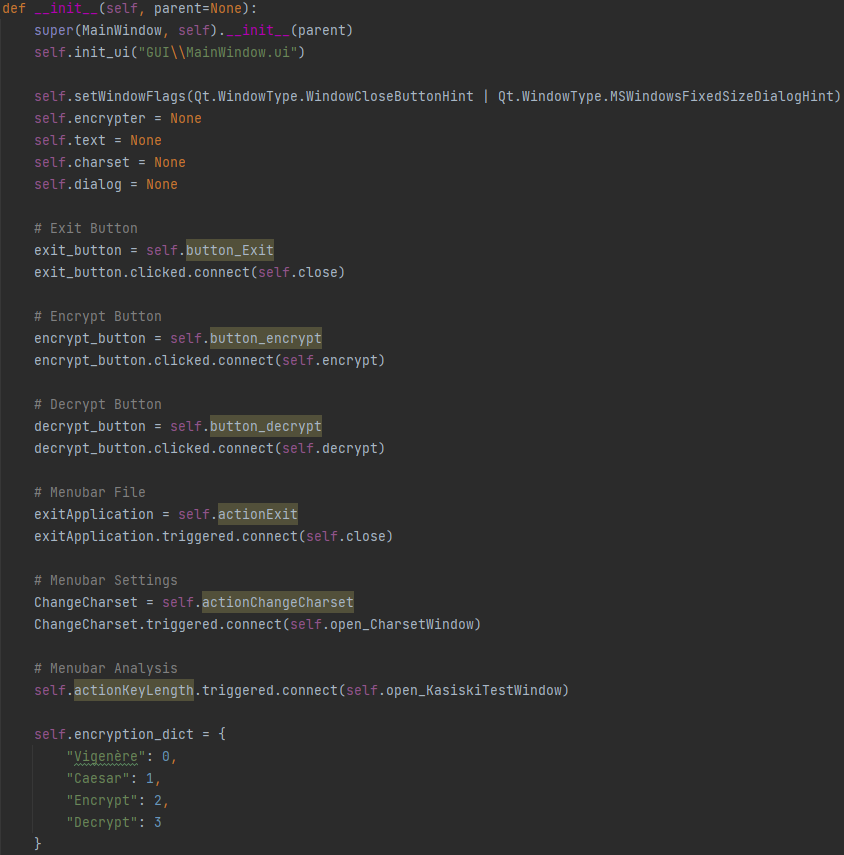
\includegraphics[width=15cm]{bilder/CodeSmells2.png}
\end{center}

\subsubsection{Code Smells 3 Large Class}
Der dritte Code Smells zeigt eine 'Large Class'. Dieser bezeichnet eine große Klasse die unter anderem zu viele Instanzvariablen, Methoden oder allgemein Codezeilen aufweist. Als Beispiel dafür ist in der unteren Abbildung die MainWindow-Klasse zu sehen.
\begin{center}
	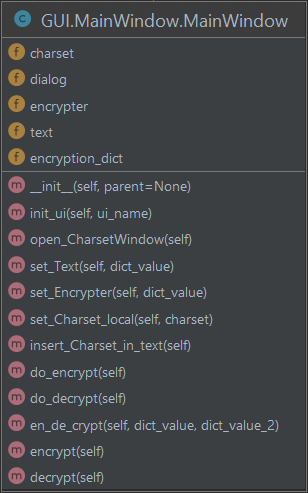
\includegraphics[width=5cm]{bilder/CodeSmells3.png}
\end{center}
Mit ~130 Zeilen Code und 10 verschiedenen Funktionen ist der Umfang der Klasse etwas zu groß. Abhilfe könnte geschaffen werden indem man beispielsweise einige Funktionen die die Handhabung der Verschlüsselung übernehmen in eine neue View-Klasse auslagert o.Ä.

\subsection{Angewendete Refactorings}
Die beiden durchgeführten Refactorings beziehen sich auf andere Beispiele als oben besprochen.

\subsubsection[Refactoring 1 Extract Method]{Refactoring 1 Extract Method\protect\footnote{Commit: \href{https://github.com/NicoSchrodt/EncryptionService/commit/5eb9481d0b440b72332d2c3ed4208e68343f3ac4}{5eb9481d0b440b72332d2c3ed4208e68343f3ac4}}}
Platzhalter

\subsubsection[Refactoring 2 Replace Error Code with Exception]{Refactoring 2 Replace Error Code with Exception\protect\footnote{Commit: \href{https://github.com/NicoSchrodt/EncryptionService/commit/e7bfbe622070be07df80dcd3635307d828a1e895}{e7bfbe622070be07df80dcd3635307d828a1e895}}}
Die Aufgabe dieses Refactorings ist es potentielle Fehler zu vermeiden die beim Fehlinterpretieren von Rückgabewerten o.Ä. auftreten können. Ziel ist es, dass ein Fehlerstatus explizit eine Exception auslöst. Dieses Refactoring wurde im Code für das Kasiski-Verfahren angewendet, dass je nach Länge des Textes keine Schlüssellänge ermitteln kann.
\begin{center}
	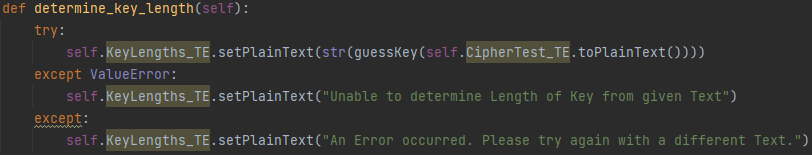
\includegraphics[width=15cm]{bilder/Refactoring2_b.png}
	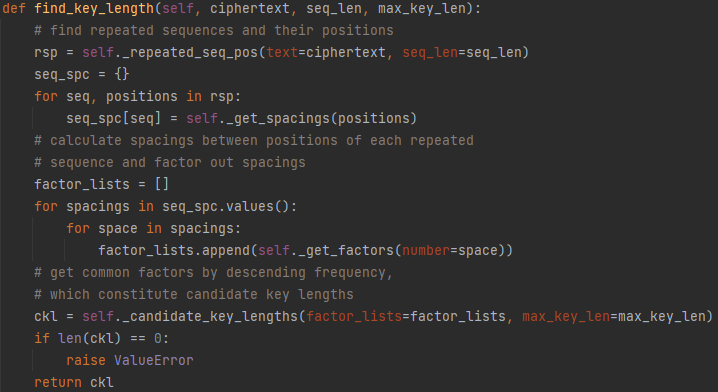
\includegraphics[width=15cm]{bilder/Refactoring2_a.png}
\end{center}
Für den Fall das die Funktion '\_candidate\_key\_lengths' eine leere Liste zurückgibt, wird statt einer Fehlermeldung ein ValueError ausgelöst. Dieser wird in der aufrufenden Funktion der Benutzeroberfläche abgefangen und entsprechend verarbeitet.
\newpage

\section{Unit Tests}
Die Aufgabe von Unit Tests ist es einen jeweils möglichst kleinen Teil eines Systems zu testen. Dabei sollen nur relevante Teile des Systems im Test verwendet werden. Bestehen Abhängigkeiten zu anderen Teilen des Systems, so werden diese mit Stellvertreterobjekten besetzt. Ziel dieser Tests ist das Sicherstellen der Funktionalität der einzelnen Komponenten.

\subsection{Verwendete Unit Tests und getesteter Code}
Um den Umfang der Tests möglichst überschaubar zu halten wurden lediglich die Funktionen der Logik-Schicht getestet. Insbesondere die Verschlüsselung, aber auch die darin relevanten Charset- und Interface Klassen erhielten UnitTests.
\begin{center}
	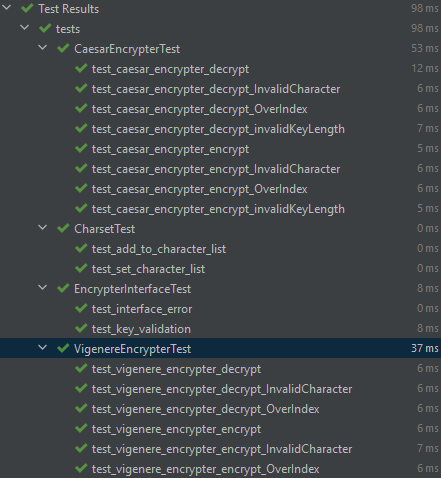
\includegraphics[width=10cm]{bilder/Tests.png}
\end{center}

\subsubsection{Mocks}
Für einige UnitTests ist es nicht möglich die einzelne Komponente abgekoppelt vom Rest zu testen. Um trotz dieser Abhängigkeiten zu anderen Klassen, Methoden, etc. die Funktionalität mit einem UnitTest sicherzustellen, werden Mocks eingesetzt. Deren Aufgabe ist es die benötigten Abhängigkeiten zu imitieren und die benötigten Schnittstellen zur Verfügung zu stellen. In diesem Projekt wurden Mocks auf zwei verschiedene Arten eingesetzt. In der unteren Abbildung ist die herkömmliche Art zu sehen.
\begin{center}
	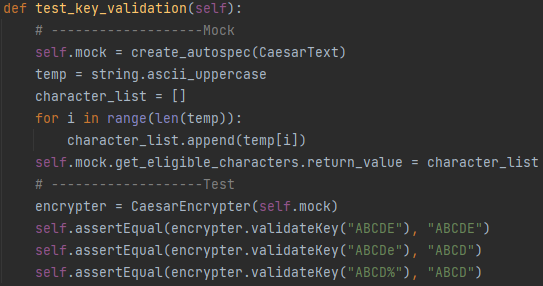
\includegraphics[width=10cm]{bilder/Mocks1.png}
\end{center}
Spezifisch für Python wird die 'create\_autospec' Funktion auf die benötigte Klasse angewendet um ein Mock-Objekt zu erzeugen, welches die Eigenschaften der Klasse annimmt. Daraufhin wird für den Mock festgelegt was die später aufgerufenen Funktionen für einen Rückgabewert haben sollen. Zum Schluss wird der Mock im Test verwendet an der Stelle an der normalerweise die Ursprungsklasse verwendet werden sollte.\\
Die zweite Art wie Mocks in den UnitTests in diesem Projekt verwendet werden ist in der nächsten Abbildung zu sehen.
\begin{center}
	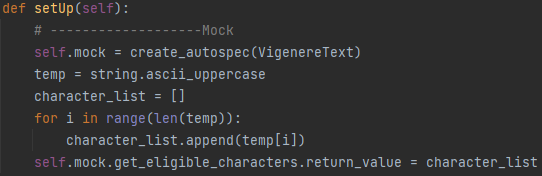
\includegraphics[width=10cm]{bilder/Mocks2.png}
\end{center}
Das Erzeugen und 'trainieren' des Mocks ist gleich wie im oberen Beispiel. Der Unterschied ist hierbei wie der Mock verwendet wird. Statt einen benötigten Mock für jeden Test individuell neu zu erzeugen und zu trainieren um ihn am Ende wieder zu verwerfen, kann man Tests mit ähnlichen Startbedingungen auch bündeln. Benötigen mehrere Tests die selben Mockobjekte, so bietet es sich an die 'setUp'-Methode zu verwenden. In einem Testbündel wird dadurch für jeden Test, vor der Ausführung dessen, diese Funktion einmal ausgeführt. Dadurch erhält man für jeden Test die selben Mocks, man spart sich aber Codeduplikate, also weniger potentielle Fehler und eine erhöhte Übersichtlichkeit. 
\subsubsection[Code Coverage]{Code Coverage\protect\footnote{Commit: 759310aada67666e973e748275b2739f1c93ace5}}
Code Coverage beschreibt, welchen Anteil der Codezeilen im gesamten Projekt von Tests durchlaufen werden. Die Aufgabe dieses Wertes ist es einen groben Überblick darüber zu geben, wie viel des Gessamtprojekts resistent gegenüber zukünftigen fehlerhaften Änderungen ist. Wichtig ist dabei aber nicht nur der absolute Prozentsatz sondern auch die Abdeckung der verschiedenen Branches einer Klasse, da nicht jede Stelle im Code gleich wichtig ist bzw. gleich oft aufgerufen wird. Mit den für dieses Projekt geschriebenen UnitTests wurde ein Coverage Report erzeugt, welcher in der unteren Abbildung zu sehen ist (Gefiltert nach eigenen Klassen).
\begin{center}
	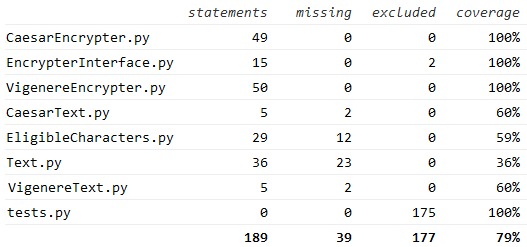
\includegraphics[width=12cm]{bilder/Coverage.png}
\end{center}
Wie zu erkennen ist werden nur die für die Logik verantwortlichen Klassen in der Coverage berücksichtigt. Weiterhin werden einige Zeilen vollständig in der Coverage verworfen. Dazu zählt beispielsweise auch die Klasse die für die Tests verantwortlich ist oder das EncrypterInterface in dem einige Zeilen lediglich eine 'NotImplemented'-Exception auslösen.
\subsection{Anwendung der ATRIP-Regeln}
Platzhalter


%\newpage
%\thispagestyle{empty}
%
%\section*{Anhang}
%\addcontentsline{toc}{section}{Anhang}


\end{document}
